% Options for packages loaded elsewhere
\PassOptionsToPackage{unicode}{hyperref}
\PassOptionsToPackage{hyphens}{url}
%
\documentclass[
  english,
  man,floatsintext]{apa6}
\usepackage{lmodern}
\usepackage{amssymb,amsmath}
\usepackage{ifxetex,ifluatex}
\ifnum 0\ifxetex 1\fi\ifluatex 1\fi=0 % if pdftex
  \usepackage[T1]{fontenc}
  \usepackage[utf8]{inputenc}
  \usepackage{textcomp} % provide euro and other symbols
\else % if luatex or xetex
  \usepackage{unicode-math}
  \defaultfontfeatures{Scale=MatchLowercase}
  \defaultfontfeatures[\rmfamily]{Ligatures=TeX,Scale=1}
\fi
% Use upquote if available, for straight quotes in verbatim environments
\IfFileExists{upquote.sty}{\usepackage{upquote}}{}
\IfFileExists{microtype.sty}{% use microtype if available
  \usepackage[]{microtype}
  \UseMicrotypeSet[protrusion]{basicmath} % disable protrusion for tt fonts
}{}
\makeatletter
\@ifundefined{KOMAClassName}{% if non-KOMA class
  \IfFileExists{parskip.sty}{%
    \usepackage{parskip}
  }{% else
    \setlength{\parindent}{0pt}
    \setlength{\parskip}{6pt plus 2pt minus 1pt}}
}{% if KOMA class
  \KOMAoptions{parskip=half}}
\makeatother
\usepackage{xcolor}
\IfFileExists{xurl.sty}{\usepackage{xurl}}{} % add URL line breaks if available
\IfFileExists{bookmark.sty}{\usepackage{bookmark}}{\usepackage{hyperref}}
\hypersetup{
  pdftitle={Satisfying housework division? Gender role beliefs and religion as moderators of housework division and satisfaction},
  pdfauthor={Carlotta Reinhardt1, Margaret Bassney1, \& Anushree Goswami1},
  pdflang={en-EN},
  hidelinks,
  pdfcreator={LaTeX via pandoc}}
\urlstyle{same} % disable monospaced font for URLs
\usepackage{graphicx,grffile}
\makeatletter
\def\maxwidth{\ifdim\Gin@nat@width>\linewidth\linewidth\else\Gin@nat@width\fi}
\def\maxheight{\ifdim\Gin@nat@height>\textheight\textheight\else\Gin@nat@height\fi}
\makeatother
% Scale images if necessary, so that they will not overflow the page
% margins by default, and it is still possible to overwrite the defaults
% using explicit options in \includegraphics[width, height, ...]{}
\setkeys{Gin}{width=\maxwidth,height=\maxheight,keepaspectratio}
% Set default figure placement to htbp
\makeatletter
\def\fps@figure{htbp}
\makeatother
\setlength{\emergencystretch}{3em} % prevent overfull lines
\providecommand{\tightlist}{%
  \setlength{\itemsep}{0pt}\setlength{\parskip}{0pt}}
\setcounter{secnumdepth}{-\maxdimen} % remove section numbering
% Make \paragraph and \subparagraph free-standing
\ifx\paragraph\undefined\else
  \let\oldparagraph\paragraph
  \renewcommand{\paragraph}[1]{\oldparagraph{#1}\mbox{}}
\fi
\ifx\subparagraph\undefined\else
  \let\oldsubparagraph\subparagraph
  \renewcommand{\subparagraph}[1]{\oldsubparagraph{#1}\mbox{}}
\fi
% Manuscript styling
\usepackage{upgreek}
\captionsetup{font=singlespacing,justification=justified}

% Table formatting
\usepackage{longtable}
\usepackage{lscape}
% \usepackage[counterclockwise]{rotating}   % Landscape page setup for large tables
\usepackage{multirow}		% Table styling
\usepackage{tabularx}		% Control Column width
\usepackage[flushleft]{threeparttable}	% Allows for three part tables with a specified notes section
\usepackage{threeparttablex}            % Lets threeparttable work with longtable

% Create new environments so endfloat can handle them
% \newenvironment{ltable}
%   {\begin{landscape}\begin{center}\begin{threeparttable}}
%   {\end{threeparttable}\end{center}\end{landscape}}
\newenvironment{lltable}{\begin{landscape}\begin{center}\begin{ThreePartTable}}{\end{ThreePartTable}\end{center}\end{landscape}}

% Enables adjusting longtable caption width to table width
% Solution found at http://golatex.de/longtable-mit-caption-so-breit-wie-die-tabelle-t15767.html
\makeatletter
\newcommand\LastLTentrywidth{1em}
\newlength\longtablewidth
\setlength{\longtablewidth}{1in}
\newcommand{\getlongtablewidth}{\begingroup \ifcsname LT@\roman{LT@tables}\endcsname \global\longtablewidth=0pt \renewcommand{\LT@entry}[2]{\global\advance\longtablewidth by ##2\relax\gdef\LastLTentrywidth{##2}}\@nameuse{LT@\roman{LT@tables}} \fi \endgroup}

% \setlength{\parindent}{0.5in}
% \setlength{\parskip}{0pt plus 0pt minus 0pt}

% Overwrite redefinition of paragraph and subparagraph by the default LaTeX template
% See https://github.com/crsh/papaja/issues/292
\makeatletter
\renewcommand{\paragraph}{\@startsection{paragraph}{4}{\parindent}%
  {0\baselineskip \@plus 0.2ex \@minus 0.2ex}%
  {-1em}%
  {\normalfont\normalsize\bfseries\itshape\typesectitle}}

\renewcommand{\subparagraph}[1]{\@startsection{subparagraph}{5}{1em}%
  {0\baselineskip \@plus 0.2ex \@minus 0.2ex}%
  {-\z@\relax}%
  {\normalfont\normalsize\itshape\hspace{\parindent}{#1}\textit{\addperi}}{\relax}}
\makeatother

% \usepackage{etoolbox}
\makeatletter
\patchcmd{\HyOrg@maketitle}
  {\section{\normalfont\normalsize\abstractname}}
  {\section*{\normalfont\normalsize\abstractname}}
  {}{\typeout{Failed to patch abstract.}}
\patchcmd{\HyOrg@maketitle}
  {\section{\protect\normalfont{\@title}}}
  {\section*{\protect\normalfont{\@title}}}
  {}{\typeout{Failed to patch title.}}
\makeatother

\usepackage{xpatch}
\makeatletter
\xapptocmd\appendix
  {\xapptocmd\section
    {\addcontentsline{toc}{section}{\appendixname\ifoneappendix\else~\theappendix\fi\\: #1}}
    {}{\InnerPatchFailed}%
  }
{}{\PatchFailed}
\usepackage{lineno}

\linenumbers
\usepackage{csquotes}
\usepackage[titles]{tocloft}
\cftpagenumbersoff{figure}
\renewcommand{\cftfigpresnum}{\itshape\figurename\enspace}
\renewcommand{\cftfigaftersnum}{.\space}
\setlength{\cftfigindent}{0pt}
\setlength{\cftafterloftitleskip}{0pt}
\settowidth{\cftfignumwidth}{Figure 10.\qquad}
\cftpagenumbersoff{table}
\renewcommand{\cfttabpresnum}{\itshape\tablename\enspace}
\renewcommand{\cfttabaftersnum}{.\space}
\setlength{\cfttabindent}{0pt}
\setlength{\cftafterloftitleskip}{0pt}
\settowidth{\cfttabnumwidth}{Table 10.\qquad}
\ifxetex
  % Load polyglossia as late as possible: uses bidi with RTL langages (e.g. Hebrew, Arabic)
  \usepackage{polyglossia}
  \setmainlanguage[]{english}
\else
  \usepackage[shorthands=off,main=english]{babel}
\fi

\title{Satisfying housework division? Gender role beliefs and religion as moderators of housework division and satisfaction}
\author{Carlotta Reinhardt\textsuperscript{1}, Margaret Bassney\textsuperscript{1}, \& Anushree Goswami\textsuperscript{1}}
\date{}


\shorttitle{gender roles, housework and satisfaction}

\affiliation{\vspace{0.5cm}\textsuperscript{1} Smith College}

\begin{document}
\maketitle

\hypertarget{analysis-strategy}{%
\subsection{Analysis Strategy}\label{analysis-strategy}}

To test our hypotheses that gender role beliefs moderate the relationship between housework distribution and satisfaction with the distribution, we used multilevel modeling and the Actor-Partner Interdependence Model (APIM; Kenny, Kashy, \& Cook, 2006). The APIM measures the effect of the explanatory variable for both members in a dyad at the same time. This way we get both the actor and partner effects. We will be able to see how one partners housework distribution effects both their own satisfaction with the distribution and their partners satisfaction with the distributions. In terms of moderation, we will get an actor effect moderated by each members gender role beliefs and a partner effect moderated by each members gender role beliefs. The APIM measures proportion of variance in satisfaction that occurs between dyads vs the total variation present. In other words, how much of the variation in satisfaction is caused by the dyad. This allows us to estimate satisfaction with the distribution of housework is a function of both housework distribution and the the random errors at both the individual and dyad level. This accounts for the nonindependent data.
In order to calculate our APIM's we had to put our data into a paired data structure, where both the actor and the partner's data was contained all in one line. This way we could calculate the actor and partner effects for both the husbands and wives.



\begin{figure}
\centering
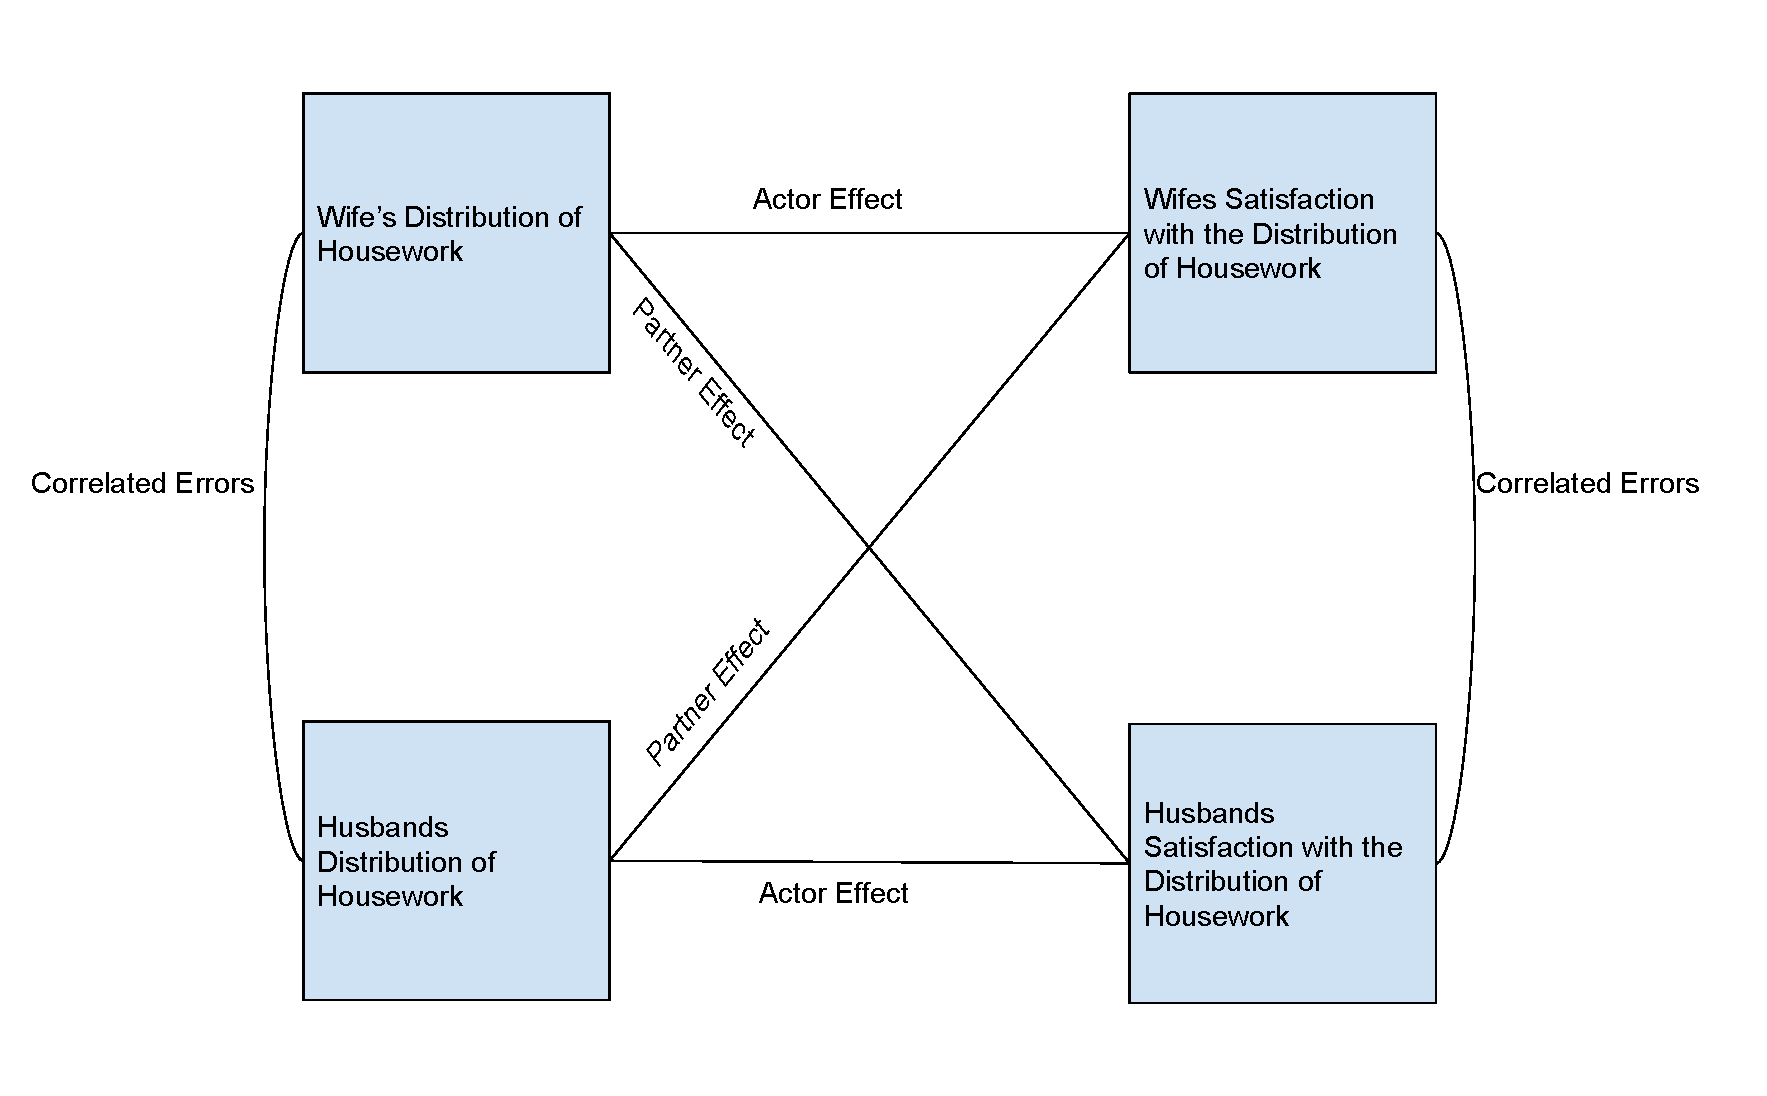
\includegraphics{APIM_Housework_Distribution.pdf}
\caption{\label{fig:my-figure}Actor Partner Effects in the APIM}
\end{figure}

\hypertarget{main-results}{%
\subsection{Main Results}\label{main-results}}

\textbf{Outcome: {[}housework\_satisfied\_A{]} Satisfaction }
\textbf{Predictor Variables: {[}avg\_housework\_female\_A,avg\_housework\_female\_P{]} Avg} \textbf{housework distribution(female tasks) of the actor and the partner}

Wife's house work distribution on her own satisfaction with the housework distribution was 0.25. Wife's house work distribution on her husbands satisfaction with the housework distribution was 0.00.Husband's house work distribution on his own satisfaction with the housework distribution was -0.03. Husband's house work distribution on his wife's satisfaction with the housework distribution was -0.01.

\textbf{Outcome: {[}housework\_satisfied\_A{]} Satisfaction}
\textbf{Predictor Variables: {[}avg\_housework\_female\_A,avg\_housework\_female\_P{]} Avg} \textbf{housework distribution(female tasks) of the actor and the partner }
\textbf{Moderators: {[}avg\_grbs\_A, avg\_grbs\_P{]} Gender role beleifs of the actor and the partner }

We found four significant parameter estimates. Only two of which were moderation effects.

The interaction between the actors gender and housework distribution and gender role beliefs was significant when the actor was the husband

estimate 0.0686374108
p-val 4.776644e-04

positive effect on satisfaction with the more housework he does, if his gender role beleifs are more traditional

The interaction between the actors gender, the actors house work distribution, and their partners gender role beliefs were significant when the actor was the husband.

estimate -0.0669358877
p-val 1.066857e-03

negative effect on satisfaction with the more housework he does, if his partners gender role beliefs are more traditional

the other two effects were just the effect of being male and the effect of being female on satisfaction.

Only looking at the three way interactions with gender we found two significant gender differences in the moderation effects.

The interaction between actors housework distribution and their own gender role beliefs was significantly different for husbands and wives

estimate 0.062986556
p-val 3.154078e-02

as the actors housework distribution increases, and their gender role beleifs are more traditional, satisfaction tended to be 0.062986556 higher for husbands than wives.

The interaction between actors housework distribution and their partners gender role beliefs was significantly different for husbands and wives

estimate -0.077597303
p-val 7.190096e-03

as the actors housework distribution increases, and their partners gender role beliefs are more traditional, satisfaction tended to be 0.077597303 lower for husbands than wives.

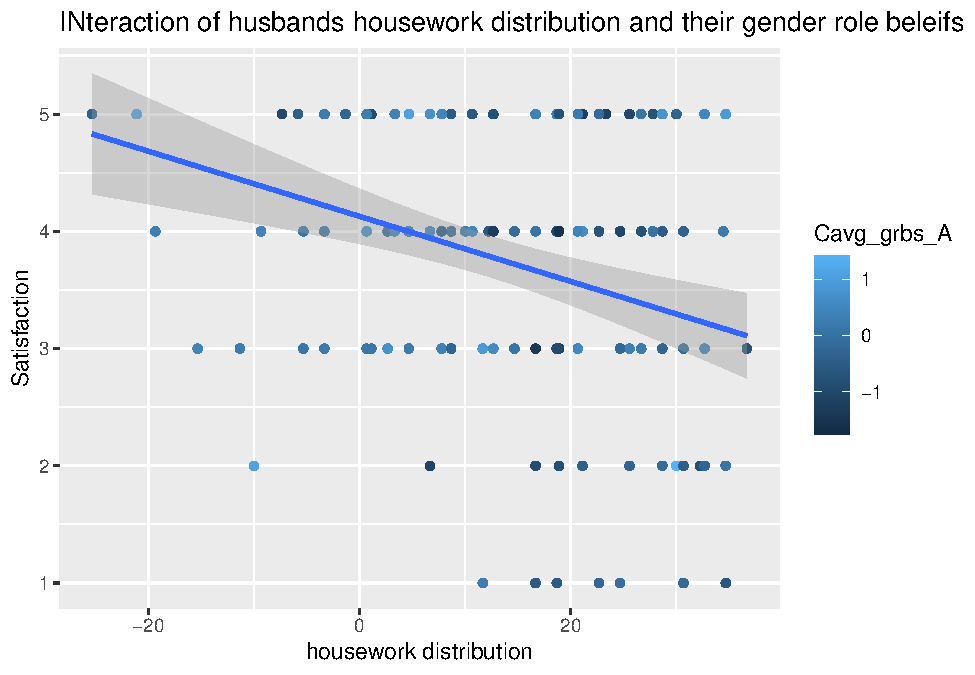
\includegraphics{results_files/figure-latex/unnamed-chunk-9-1.pdf}

\textbf{Outcome: {[}housework\_satisfied\_A{]} Satisfaction}
\textbf{Predictor Variables: {[}avg\_housework\_female\_A,avg\_housework\_female\_P{]} Avg} \textbf{housework distribution(female tasks) of the actor and the partner }
\textbf{Moderators: {[}religionYN\_A,religionYN\_P{]} Gender role beleifs of the actor and the partner }

The two intercept model gives us the two coefficients for men and women

\hypertarget{exploratory-results}{%
\subsection{Exploratory Results}\label{exploratory-results}}


\clearpage
\renewcommand{\listfigurename}{Figure captions}

\clearpage
\renewcommand{\listtablename}{Table captions}


\end{document}
